\chapter{Análisis y Desarrollo Experimental}\label{ch:analisis-y-desarrollo-experimental}
En este capítulo se recoge el estudio de técnicas del DL para el diagnóstico del Alzheimer, pasando por las 
herramientas y los datos utilizados hasta la experimentación y el análisis de los resultados obtenidos.

\section{Presentación del problema a resolver}\label{sec:presentacion-del-problema-a-resolver}
Tras la investigación del estado actual de la literatura en este ámbito, se recopilan los siguientes puntos sobre el DL
para clasificación de la EA:

\begin{itemize}
    \item El Transfer Learning es la mejor técnica de entrenamiento.
    \item Los datasets balanceados ofrecen mejores resultados, y más fiables, en la clasificación de imágenes,
    pero la limitación de disponibilidad de biomarcadores del seguimiento de la EA puede suponer un obstáculo.
    \item La prueba más frecuente para el diagnóstico de la enfermedad es la MRI.
    \item No se clarifica qué plano cerebral (axial, coronal o sagital) es mejor utilizar y bajo qué diferencias de
    rendimiento.
    \item No se realizan comparativas de rendimiento entre distinto número de clases. \\
\end{itemize}

Se propone desarrollar un sistema de aprendizaje profundo a partir de MRI con el cual:

\begin{itemize}
    \item Realizar un análisis sobre qué plano cerebral ofrece mejores resultados en el diagnóstico de la EA, ya que se
    tiene en cuenta que las redes neuronales de 3 dimensiones requieren de una capacidad computacional muy alta.
    \item Realizar una comparativa del rendimiento de la clasificación entre 2 y 3 clases: Cognitivamente normal frente 
    a Alzheimer y cognitivamente normal frente a deterioro cognitivo leve frente Alzheimer. \\
\end{itemize}

\section{Conjunto de datos empleado}\label{sec:conjunto-de-datos-empleado}
El conjunto de biomarcadores MRI que se ha utilizado se ha obtenido de la base de datos ADNI, que es un estudio
longitudinal multicéntrico en el que se desarrollan biomarcadores genéticos, bioquímicos y de imagen para la detección
temprana y el seguimiento de la EA, se habla más en profundidad sobre esta base de datos en el
apartado~\ref{ch:aped.a}.
Cabe destacar que también intentó hacer uso de la base de datos OASIS, de forma que se obtuviera un número mayor de
datos y poder prevenir los posibles problemas por falta de datos, pero no fue posible ya que no se aprobó la solicitud
de acceso realizada.

Para la selección de los biomarcadores MRI a utilizar se han dividido 3 grupos de investigación según el grado de EA
del sujeto, diferenciándose:
\begin{itemize}
    \item \textbf{Cognitivamente normal} (en adelante este grupo se denominará \textbf{CN}): Sujetos sanos.
    \item Sujetos con un \textbf{deterioro cognitivo leve}, del inglés Mild Cognitive Impairment (en adelante este grupo
    se denominará \textbf{MCI})
    \item Sujetos con \textbf{Alzheimer} diagnosticado (en adelante este grupo se denominará \textbf{AD}). \\
\end{itemize}

Para la realización de la experimentación se han utilizado biomarcadores MRI de tipo \textit{NIfTI} pertenecientes a un
subconjunto de datos sometidos a un post-procesamiento que se comenta en la sección~\ref{subsec:post-procesamiento-en-adni}.

En el subconjunto de datos disponibles, los biomarcadores de clase AD son más limitados que los de clase CN y MCI.
Siendo la distribución de los datos la siguiente:

\begin{figure}[H]
    \centering
    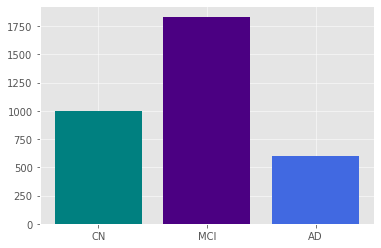
\includegraphics[width=0.6\textwidth]{./imgs/histograma-de-clases}
    \caption{Histograma de clases}
    \label{fig:histograma-de-clases}
\end{figure}

Como se puede apreciar en la Figura~\ref{fig:histograma-de-clases}, existe un desbalance de clases, habiendo 998
neuroimágenes de tipo CN, 1832 de tipo MCI y 602 de tipo AD.

Para realizar el entrenamiento con un datasets balanceado se utilizan todos los datos de tipo AD disponibles y se
realiza un submuestreo de las clases mayoritarias para equilibrar las clases.
El uso de la técnica de submuestreo presenta una desventaja ya que se pierde información, pero se elige esta técnica
frente a la técnica de sobremuestreo, ya que esta última consiste en aumentar los datos de la clase minoritaria, lo
que puede llevar a un sobreajuste y teniendo en cuenta que ya el conjunto de datos general del que se dispone es muy
limitado y es posible que se obtenga un sobreajuste no se quieren multiplicar las posibilidades.

De modo que el conjunto completo de datos balanceado que se utiliza para extraer los cortes axial, coronal y sagital
está formado por \textbf{1806} neuroimágenes en total.

\section{Herramientas utilizadas}\label{sec:herramientas-utilizadas}
Para realizar este estudio es necesario utilizar una serie de herramientas que faciliten y hagan posible la 
experimentación.
Hay que tener en cuenta dos grupos de herramientas: Las herramientas para trabajar con biomarcadores de tipo MRI y las 
herramientas para trabajar con técnicas de DL.

\subsection{Herramientas para trabajar con biomarcadores MRI de tipo NIfTI}
\label{subsec:herramientas-para-trabajar-con-biomarcadores-mri-de-tipo-nifti}
Para poder realizar el sistema de clasificación es necesario realizar un procesamiento de los archivos de MRI, de 
manera que se obtengan cortes de 2 dimensiones a partir del archivo en 3 dimensiones.
Para conseguirlo se ha hecho uso de la librería para python \textbf{NiBabel}, que permite la lectura y escritura  de 
archivos de neuroimagen, en nuestro caso del formato \textit{NIfTI}.
Por lo que mediante esta librería se puede cargar una MRI, extraer el corte o slice deseado y guardarlo.

Además, para la visualización de este tipo de archivos se requiere de software de visualización de imágenes específico.
Hay múltiples herramientas disponibles para ello según la finalidad que se quiera conseguir.
Para visualizar archivos en formato \textit{NIfTI} se ha hecho uso del software \textbf{MRIcron}, que ha requerido 
instalación y con el que se ha podido realizar una visualización de múltiples capas de la MRI. También se ha hecho uso 
del recurso \textbf{IDA} online del que se obtienen los datos de la base de datos \textit{ADNI} y del que se detalla más
información en el el apartado~\ref{ch:aped.a}.
Este recurso integra un visualizador de neuroimágenes.


\subsection{Herramientas para trabajar con técnicas de Deep Learning}
\label{subsec:herramientas-para-trabajar-con-tecnicas-de-deep-learning}
Como bien se muestra en el apartado~\ref{sec:datos-y-herramientas-estado-del-arte}, existe un amplio abanico de
posibilidades en cuanto a herramientas que permiten la experimentación de técnicas de DL.

De entre todas ellas se ha optado por utilizar \textbf{TensorFlow} y \textbf{Keras}, no solo por ser las más utilizadas
en la literatura, sino también porque son las que ofrecen una mejor documentación para su uso.

Para trabajar con imágenes 2D y por lo tanto con vectores y matrices se hace uso de la biblioteca de \textit{Python}
\textbf{NumPy}.

Para visualizar, tanto las imágenes de los planos cerebrales obtenidos como para la representación de las gráficas de
resultados se usa \textbf{Matplotlib}.

Para obtener las métricas para evaluar los resultados obtenidos del entrenamiento se hace uso de la librería
\textbf{scikit-learn}.

Por lo tanto el lenguaje de programación con el que se va a trabajar en este TFG y en concreto en el desarrollo
experimental es \textbf{Python}.

\section{Procesamiento de biomarcadores}\label{sec:procesamiento-de-biomarcadores}

\subsection{Post-procesamiento en ADNI}\label{subsec:post-procesamiento-en-adni}
Tal y como se ha comentado en ~\ref{sec:conjunto-de-datos-empleado}, el conjunto de datos utilizado en este estudio se
ha obtenido de un subconjunto de neuroimágenes de ADNI al que se le aplica un procesamiento, con el objetivo de extraer
la información más importante y descartar la irrelevante.

Para la realización de este procesamiento, al que ADNI denomina como post-procesamiento, ya que se  en una fase
posterior a la examinación del sujeto, se hace uso de la herramienta FreeSurfer y  se aplican las siguiente técnicas:

\begin{itemize}
    \item \textbf{Registro de la imagen}: proceso de transformación a un sistema de coordenadas común.
    Consiguiendo que en distintas imágenes cerebrales los í correspondan en posición.
    \item \textbf{Segmentación del cráneo}: proceso de eliminación del cráneo para aislar la masa cerebral.
    \item \textbf{Normalización de la intensidad}: proceso de corrección de intensidad de la imagen.
    Se aplica N3 que es un algoritmo de afilado de picos de histograma. \\
\end{itemize}

En la Figura~\ref{fig:adni-mri} se puede ver una comparativa entre una MRI en bruto con MP-RAGE y la misma post-procesada con
FreeSurfer.

\begin{figure}[H]
    \centering
    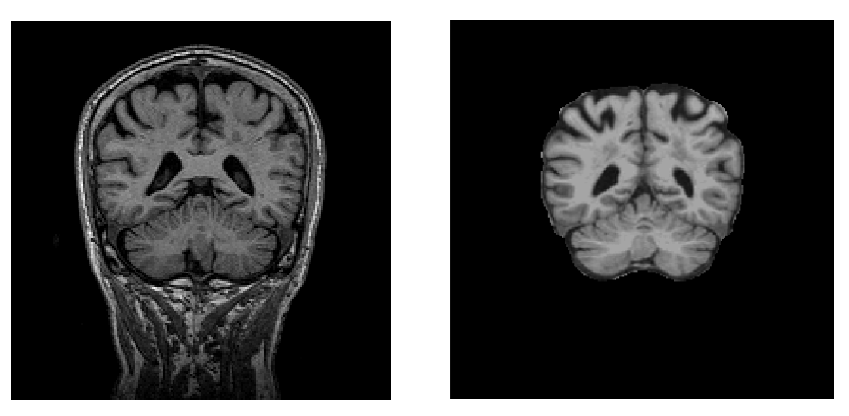
\includegraphics[width=\textwidth]{./imgs/adni-mri}
    \caption{Técnicas de procesamiento de MRI en ADNI. De izquierda a derecha: MRI en bruto con MP-RAGE y MRI
    post-procesada con FreeSurfer. Fuente: Alzheimer’s Disease Neuroimaging Initiative~\cite{img-adni-mri}. }
    \label{fig:adni-mri}
\end{figure}

\subsection{Creación de las imágenes para el entrenamiento}\label{subsec:creacion-de-las-imagenes-para-el-entrenamiento}
Para evaluar qué plano cerebral ofrece mejores resultados para el diagnóstico de la EA a partir de biomarcadores MRI es
necesario obtener imágenes 2D a partir de los archivos de MRI \textit{NIfTI}.

\begin{figure}[H]
    \centering
    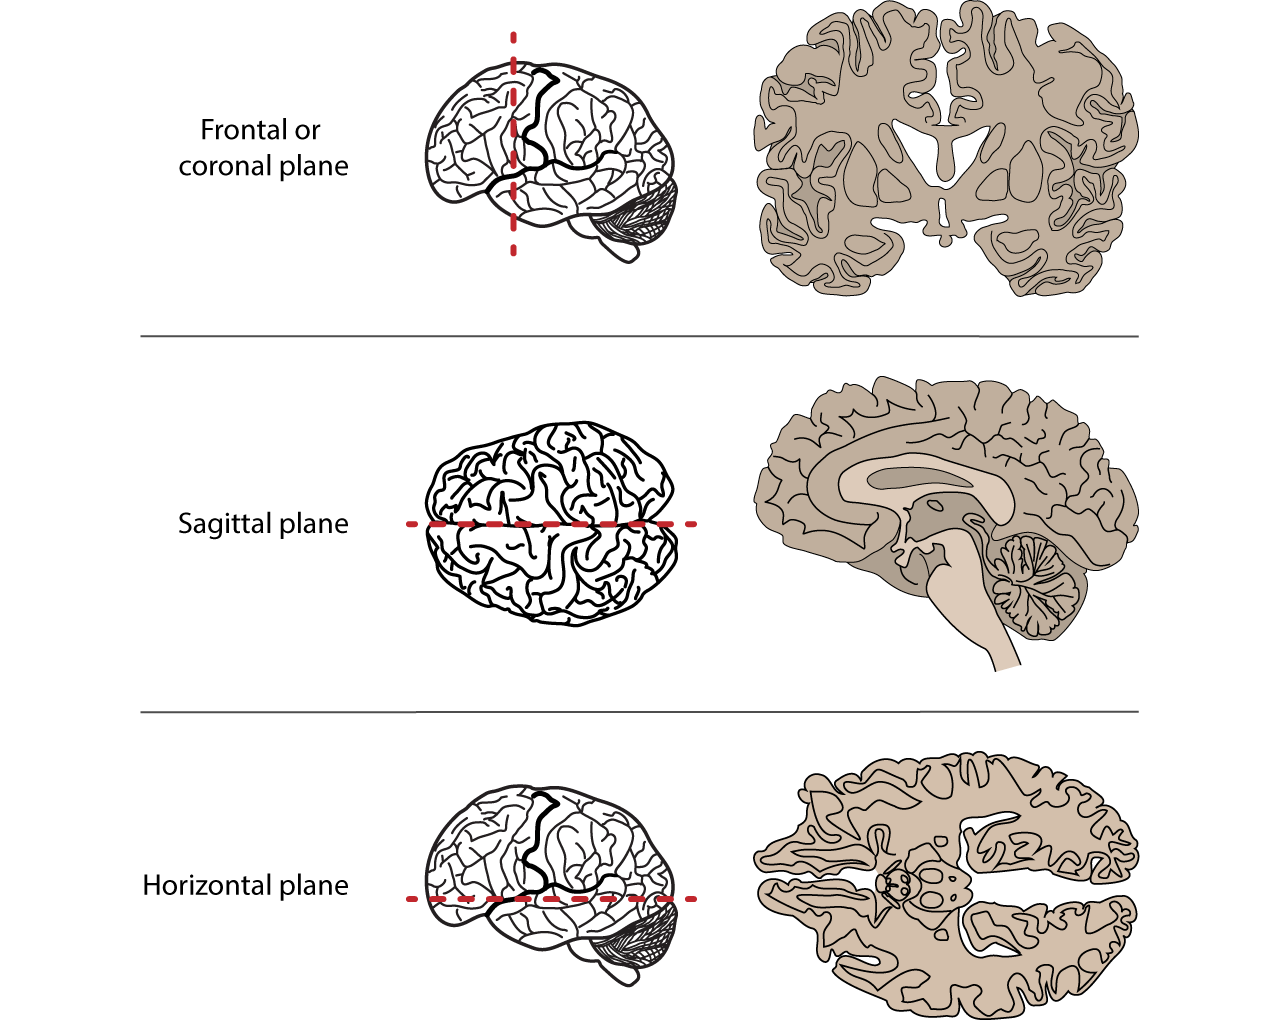
\includegraphics[width=\textwidth]{./imgs/planos-cerebrales}
    \caption{Planos Cerebrales. Fuente: Anatomical Planes por Casey Henley~\cite{img-planos-cerebrales}. }
    \label{fig:planos-cerebrales}
\end{figure}

Para ello mediante un script de python se leen las imágenes 3D, se generan los cortes correspondientes a los planos
usando la capa de central como corte del plano para extraer la mayor información posible y se guardan los cortes
generados en carpetas dedicadas a cada plano.

De manera que el conjunto de resonancias magnéticas del que se extraen los cortes es el mismo para los tres subconjuntos
que se obtienen.
De esta forma se garantiza que a la hora de concluir la evaluación, los cortes han surgido de las mismas resonancias
magnéticas y los resultados serán fiables.

\begin{figure}[H]
    \centering
    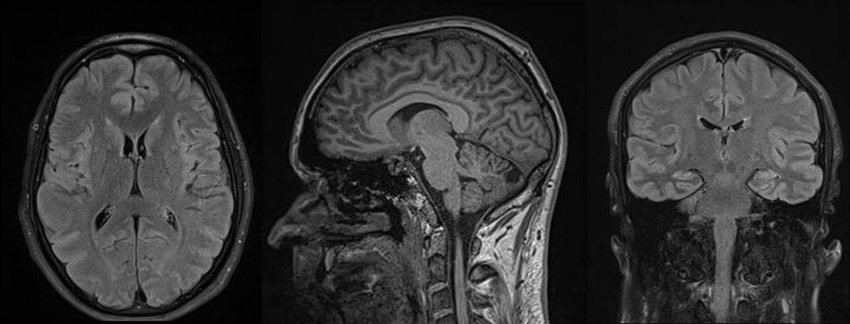
\includegraphics[width=\textwidth]{./imgs/MRI-planos-cerebrales}
    \caption{MRI en los planos axial, sagital y coronal.
    Fuente: Trakia Journal of Sciences~\cite{img-mri-planos-cerebrales}. }
    \label{fig:mri-planos-cerebrales}
\end{figure}

\section{Estrategias de entrenamiento}\label{sec:estrategias-de-entrenamiento}
Tras la conclusión de la revisión de la literatura se ha decidido aplicar en este estudio las técnicas de Transferencia
de Aprendizaje o Transfer Learning (en adelante TL) y Aumento de datos o Data Augmentation.
En este apartado se explica el fundamento de ambas técnicas.

\subsection{Transfer Learning}\label{subsec:transfer-learning}
El TL es una técnica que consiste en utilizar modelos probados y pre-entrenados, con un conjunto de datos igual o
distinto al problema a resolver, para volver a entrenarlos con el conjunto de datos relativos al problema.
De modo que se requiere menos tiempo de cálculo o recursos que si se construye el modelo desde cero.

Tal y como se ha concluido en la revisión de la literatura, esta técnica es útil y ofrece un gran número de ventajas,
por lo tanto en este estudio se ha aplicado esta técnica utilizando una arquitectura pre-entrenada con los pesos de
\textit{ImageNet}.

En cuánto a la forma de aplicar TL se ha optado por aplicar \textit{fine-tuning} ya que al utilizar esta técnica se
aprovechan las ventajas que aporta el uso de transferencia de aprendizaje para conjuntos de datos distintos a los del
entrenamiento original.
Para ello los pasos son:
\begin{itemize}
    \item Se crea el modelo base pre-entrenado.
    \item Se reconstruye la parte superior del modelo adaptándola al problema que se quiera solucionar.
    \item Se congela la base convolucional para la extracción de características.
    \item Se entrena el modelo sólo con los pesos de la última capa, de manera que se aprovechan las características
    aprendidas en la última capa para la resolución del problema.
    \item Se descongelan las capas superiores del modelo, se escoge la capa desde la que quiere aplicar
    \textit{fine-tuning} y se congelan todas las capas previas a esa.
    \item Se re-entrena el modelo durante un número de épocas con el objetivo de aumentar la precisión del modelo.\\
\end{itemize}

\subsection{Data Augmentation}\label{subsec:data-augmentation}
Esta técnica consiste en aumentar la diversidad del conjunto de entrenamiento mediante la aplicación de transformaciones
aleatorias pero realistas.

Las técnicas de aumento de datos han demostrado una mejora del rendimiento de la clasificación sin la necesidad de
recoger nuevos datos cuando estos son limitados, y teniendo en cuenta que para este estudio los datos disponibles son
reducidos, se opta por aplicarla en la experimentación.

\section{Arquitectura del modelo profundo utilizado}\label{sec:arquitectura-del-modelo-profundo-utilizado}
Se ha elegido \textbf{EfficientNetB7} como modelo pre-entrenado porque es el modelo de aprendizaje profundo pre-entrenado
con mejor rendimiento que ofrece Keras~\cite{keras-applications}.

Las \textit{EfficientNets} son una familia de modelos de clasificación de imágenes que alcanzan una alta precisión,
pero siendo en orden de magnitud más pequeños y rápidos que otros modelos~\cite{efficientnets}.

\begin{figure}[H]
    \centering
    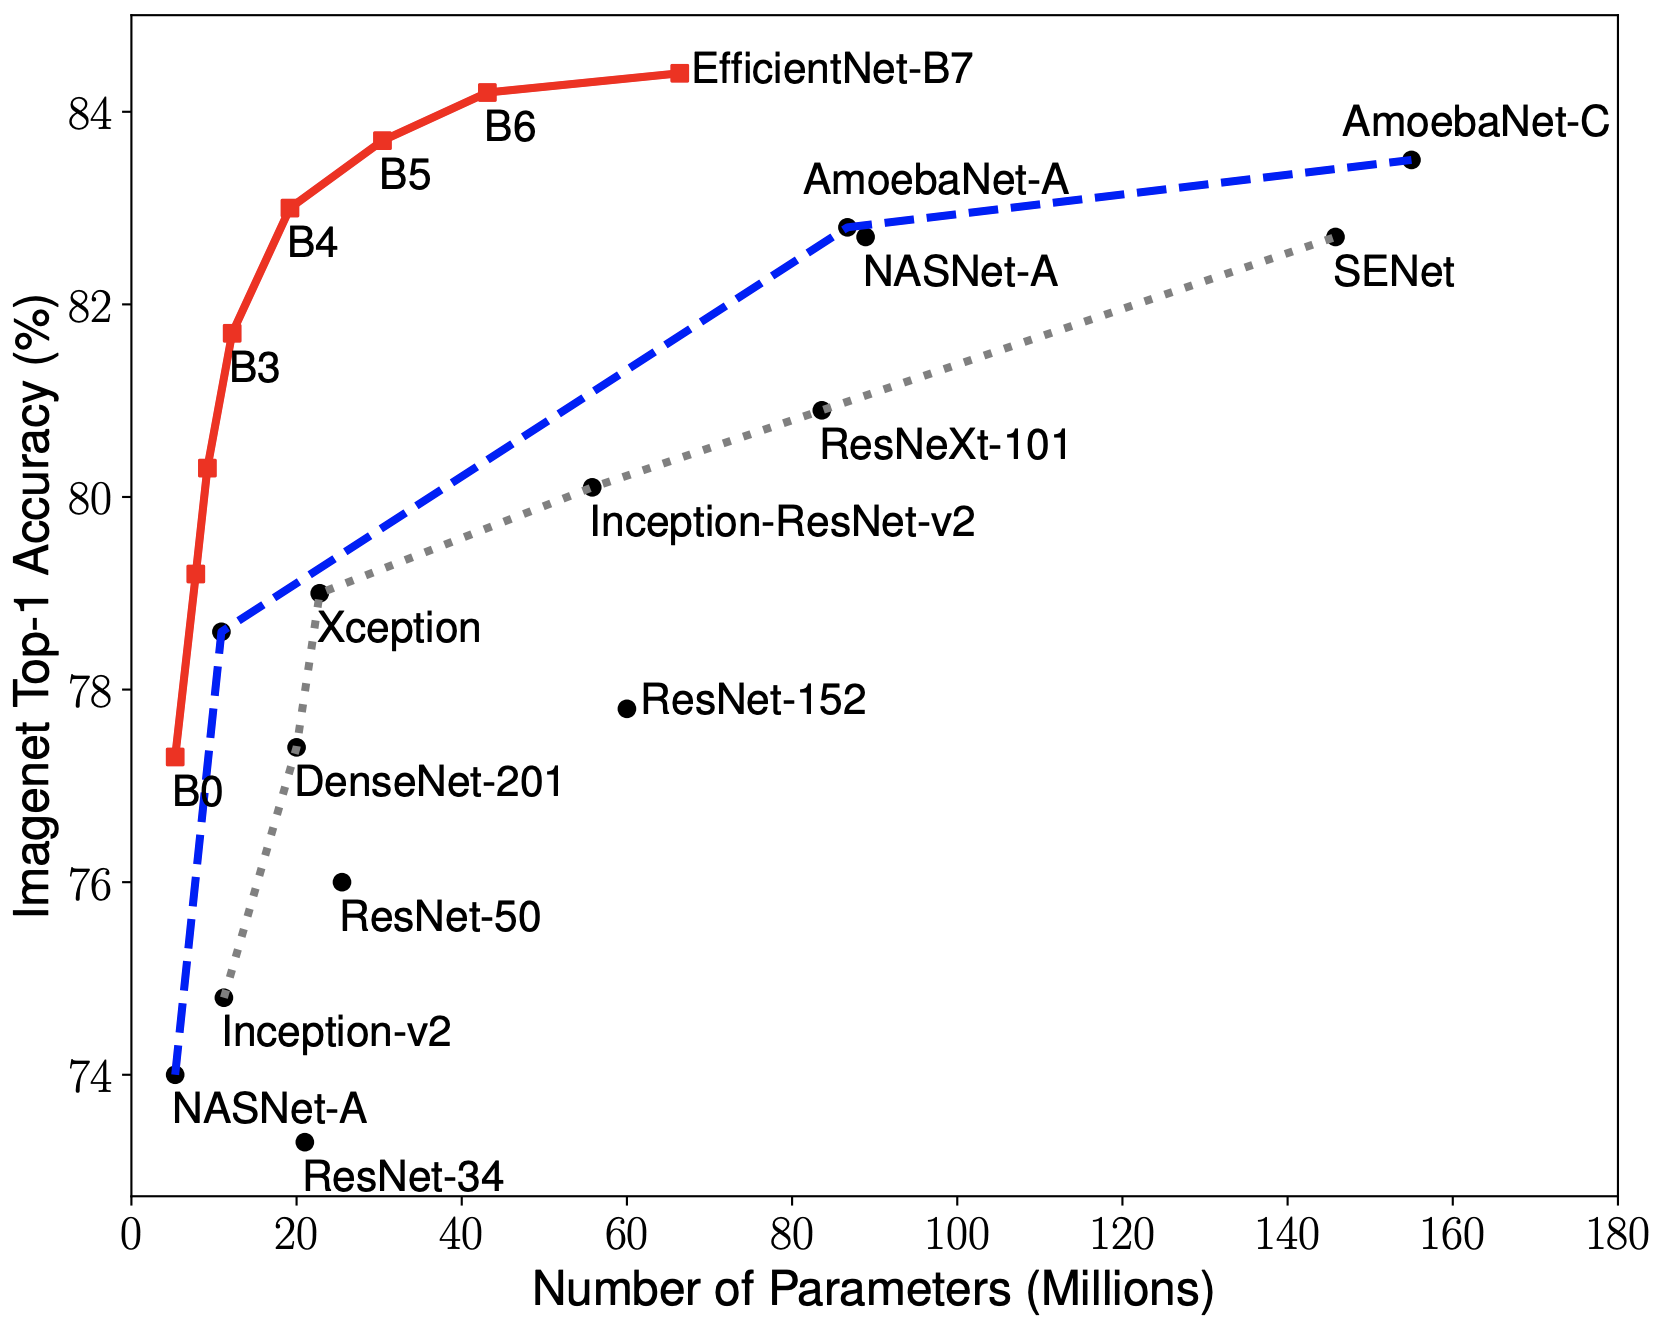
\includegraphics[width=0.5\textwidth]{./imgs/redimiento-efficientnet}
    \caption{Rendimiento de EfficientNet en comparación con otras arquitecturas. Fuente:~\cite{efficientnets-models}. }
    \label{fig:redimiento-efficientnet}
\end{figure}

\begin{figure}[H]
    \centering
    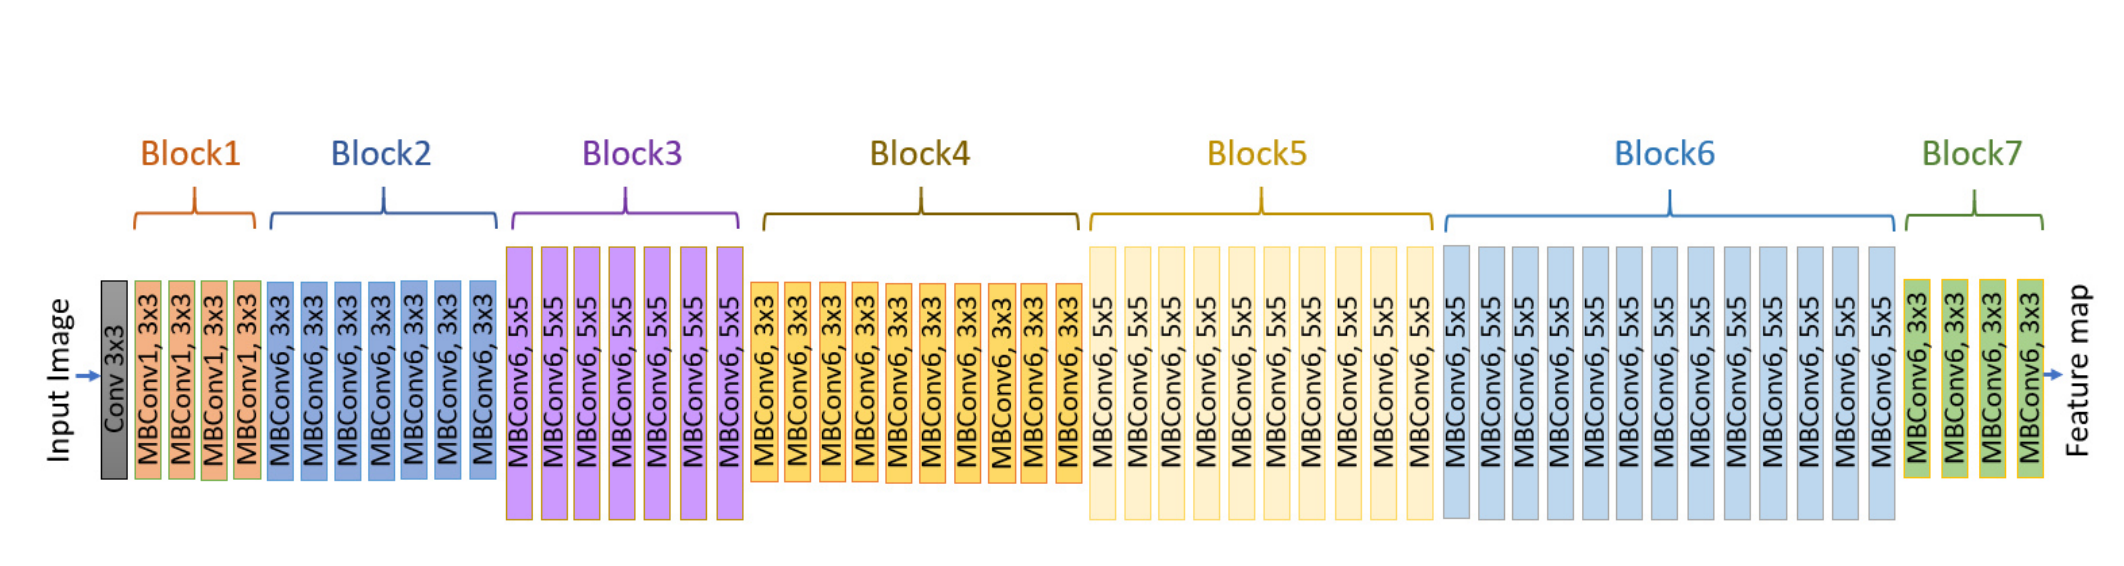
\includegraphics[width=\textwidth]{./imgs/efficientnetb7-model-architecture}
    \caption{Arquitectura del modelo EfficientNetB7. Fuente:~\cite{efficientnetb7-model-architecture}. }
    \label{fig:efficientnetb7-model-architecture}
\end{figure}

\section{Estrategia de entrenamiento}\label{sec:estrategia-de-entrenamiento}
En este caso al aplicar \textit{fine-tuning}, a la hora de reconstruir la parte superior del modelo, se han añadido las
siguientes capas con el objetivo de prevenir y reducir el \textit{overfitting} o \textit{sobreajuste}:
\begin{itemize}
    \item Capa Global Average Pooling para la regularización estructural y evitar el sobreajuste de la estructura global.
    \item Capa Dropout con un  rate de 0.3 para que nuestro modelo sea más robusto.
    \item Capa Batch Normalization para mejorar el funcionamiento, velocidad y estabilidad. \\
\end{itemize}

En cuanto a la aplicación de Data Augmentation, se ha incluido como capa de preprocesamiento del modelo formando parte
del mismo, de esta forma a la hora de exportar el modelo e implementarlo, se estandarizarán de manera automática las
imágenes evitando que haya que repetir este preprocesamiento en el lado del servidor.
Lo que resulta una ventaja de cara a la implementación de la aplicación web que forma parte de este proyecto.

Para aumentar el conjunto de entrenamiento se ha incluido una capa para rotar la imagen y otra para voltear horizontal
y verticalmente.

También se incluye en la capa de preprocesamiento del modelo un redimensionado de las imágenes a 224×224 píxeles para
no causar conflictos con la entrada del modelo base.

Al aplicar TL se han seguido los pasos comentados en el apartado~\ref{subsec:transfer-learning} y se ha utilizado de
referencia el análisis de la literatura y la documentación de Keras y TensorFlow.
De modo que se ha definido un tamaño de \textit{batch} de 32, se han establecido el número de épocas iniciales y de re-entreno
a 10, formando un total de épocas de 20 y la capa en la que se va a aplicar \textit{fine-tuning} a 20.
El valor de la tasa de aprendizaje utilizado en la primera fase se ha establecido con un rate de 0.0001 y en la segunda
fase 0.00001, haciendo uso del optimizador Adam (Adaptive moment estimation) en la primera fase y
RMSprop (Root Mean Square Propagation) en la segunda.


\section{Experimentos}\label{sec:experimentos}
En esta sección se muestran los resultados obtenidos.
Se ha utilizado el mismo modelo para hacer la comparativa, cambiando únicamente los datos de entrenamiento en base a
cada caso.

\subsection{Análisis de resultados}\label{subsec:analisis-de-resultados}
Para realizar la evaluación de los resultados y obtener una conclusión al estudio se va a utilizar de
métrica la precisión o \textit{accuracy}.

    \[accuracy=\frac{VP+VN}{VP+VN+FP+FN}\]

La precisión establece qué porcentaje de datos han sido etiquetados de forma correcta por el
Siendo o \textit{VP} y o \textit{VN} los verdaderos positivos y verdaderos negativos respectivamente,
y o \textit{FP} y o \textit{FN} los falsos positivos y falsos negativos respectivamente.

Puesto que el dataset con el que se trabaja en este estudio está balanceado esta métrica es relevante para realizar
la evaluación.

Además de cada caso se va a incluir la evolución del modelo durante el entrenamiento, la matriz de confusión y el
Informe de clasificación o o \textit{Classification Report}.


\subsection{Resultados del plano Axial}\label{subsec:resultados-del-plano-axial}

\begin{figure}[H]
    \centering
    \begin{subfigure}{0.4\textwidth}
        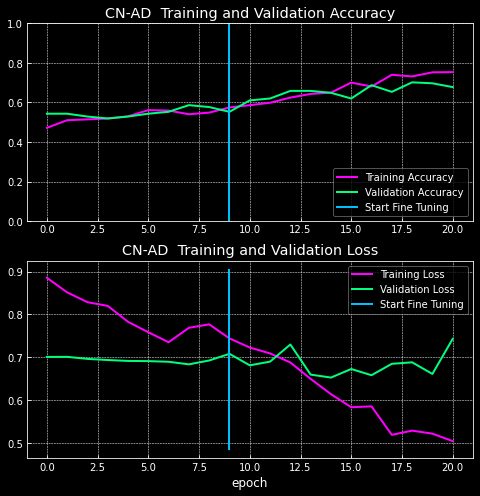
\includegraphics[width=\textwidth]{./imgs/resultados/axial/CN_AD_output_AXIAL}
        \caption{Comparativa CN-AD. }
        \label{fig:axial-cn-ad}
    \end{subfigure}
    \hspace*{\fill}
    \begin{subfigure}{0.4\textwidth}
        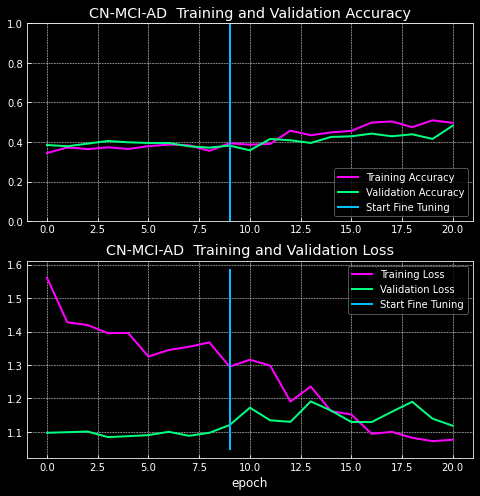
\includegraphics[width=\textwidth]{./imgs/resultados/axial/CN_MCI_AD_output_AXIAL}
        \caption{Comparativa CN-MCI-AD. }
        \label{fig:axial-c-mci-ad}
    \end{subfigure}
    \caption{Evolución del modelo durante el entrenamiento: plano Axial} \label{fig:axial-model}
\end{figure}

\begin{table}[H]
    \centering
    \begin{tabular}{r r r r r}
        & precision & recall & f1-score & support \\
        AD & 0.70 & 0.50 & 0.58 & 14 \\
        CN & 0.68 & 0.83 & 0.75 & 18 \\
        & & & & \\
        accuracy &  &  & 0.69 & 32 \\
        macro avg & 0.69 & 0.67 & 0.67 & 32 \\
        weighted avg & 0.69 & 0.69 & 0.68 & 32 \\
    \end{tabular}
    \caption{Classification Report del plano Axial. Comparativa CN-AD}
    \label{tab:cr-axial-cn-ad}
\end{table}

\begin{table}[H]
    \centering
    \begin{tabular}{r r r r r}
        & precision & recall & f1-score & support \\
        AD & 0.80 & 0.67 & 0.73 & 12 \\
        CN & 0.50 & 0.64 & 0.56 & 11 \\
        MCI & 0.25 & 0.22 & 0.24 & 9 \\
        & & & & \\
        accuracy &  &  & 0.53 & 32 \\
        macro avg & 0.52 & 0.51 & 0.51 & 32 \\
        weighted avg & 0.54 & 0.53 & 0.53 & 32 \\
    \end{tabular}
    \caption{Classification Report del plano Axial. Comparativa CN-MCI-AD}
    \label{tab:cr-axial-cn-mci-ad}
\end{table}

\begin{figure}[H]
    \centering
    \begin{subfigure}{0.4\textwidth}
        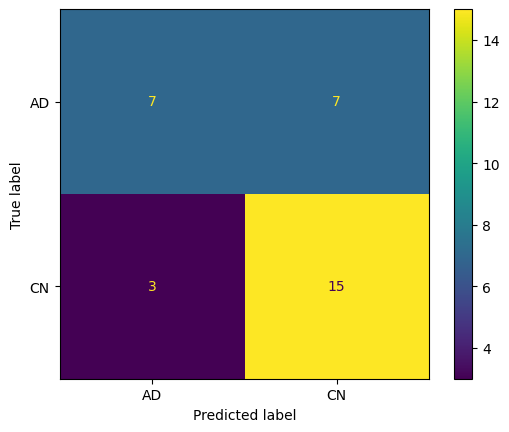
\includegraphics[width=\textwidth]{./imgs/resultados/axial/CN_AD_cm_AXIAL}
        \caption{Comparativa CN-AD. }
        \label{fig:mc-axial-cn-ad}
    \end{subfigure}
    \hspace*{\fill}
    \begin{subfigure}{0.4\textwidth}
        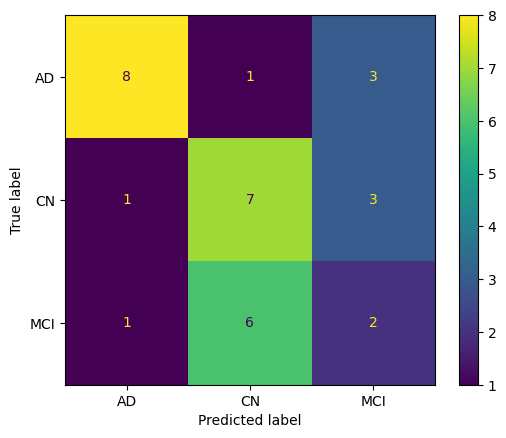
\includegraphics[width=\textwidth]{./imgs/resultados/axial/CN_MCI_AD_cm_AXIAL}
        \caption{Comparativa CN-MCI-AD. }
        \label{fig:mc-axial-cn-mci-ad}
    \end{subfigure}
    \caption{Matrices de confusión del plano Axial} \label{fig:mc-axial}
\end{figure}

Al comparar entre CN y AD en el plano axial se obtiene una precisión del 69\%
Frente al 53\% que se obtiene en la clasificación entre CN, MCI y AD. Además  en la comparación de dos clases se
observa un valor alto de falsos negativos.
En la clasificación de tres clases el etiquetado de la clase intermedia MCI ha sido  peor en comparación a CN y AD.


\subsection{Resultados del plano Coronal}\label{subsec:resultados-del-plano-coronal}

\begin{figure}[H]
    \centering
    \begin{subfigure}{0.4\textwidth}
        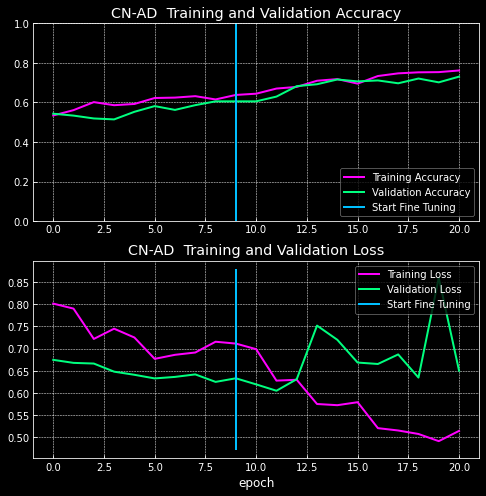
\includegraphics[width=\textwidth]{./imgs/resultados/coronal/CN_AD_output_CORONAL}
        \caption{Comparativa CN-AD. }
        \label{fig:coronal-cn-ad}
    \end{subfigure}
    \hspace*{\fill}
    \begin{subfigure}{0.4\textwidth}
        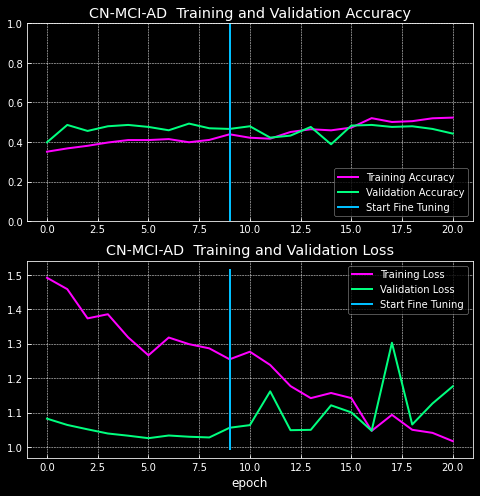
\includegraphics[width=\textwidth]{./imgs/resultados/coronal/CN_MCI_AD_output_CORONAL}
        \caption{Comparativa CN-MCI-AD. }
        \label{fig:coronal-c-mci-ad}
    \end{subfigure}
    \caption{Evolución del modelo durante el entrenamiento: plano Coronal.} \label{fig:coronal-model}
\end{figure}

\begin{table}[H]
    \centering
    \begin{tabular}{r r r r r}
        & precision & recall & f1-score & support \\
        AD & 0.83 & 0.59 & 0.69 & 17 \\
        CN & 0.65 & 0.87 & 0.74 & 15 \\
        & & & & \\
        accuracy &  &  & 0.72 & 32 \\
        macro avg & 0.74 & 0.73 & 0.72 & 32 \\
        weighted avg & 0.75 & 0.72 & 0.71 & 32 \\
    \end{tabular}
    \caption{Classification Report del plano Coronal. Comparativa CN-AD}
    \label{tab:cr-coronal-cn-ad}
\end{table}

\begin{table}[H]
    \centering
    \begin{tabular}{r r r r r}
        & precision & recall & f1-score & support \\
        AD & 0.67 & 0.50 & 0.57 & 8 \\
        CN & 0.62 & 0.50 & 0.56 & 10 \\
        MCI & 0.56 & 0.71 & 0.63 & 14 \\
        & & & & \\
        accuracy &  &  & 0.59 & 32 \\
        macro avg & 0.62 & 0.57 & 0.58 & 32 \\
        weighted avg & 0.61 & 0.59 & 0.59 & 32 \\
    \end{tabular}
    \caption{Classification Report del plano Coronal. Comparativa CN-MCI-AD}
    \label{tab:cr-coronal-cn-mci-ad}
\end{table}

\begin{figure}[H]
    \centering
    \begin{subfigure}{0.4\textwidth}
        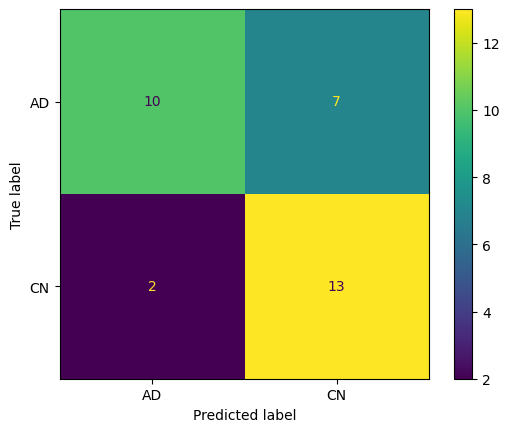
\includegraphics[width=\textwidth]{./imgs/resultados/coronal/CN_AD_cm_CORONAL}
        \caption{Comparativa CN-AD. }
        \label{fig:mc-coronal-cn-ad}
    \end{subfigure}
    \hspace*{\fill}
    \begin{subfigure}{0.4\textwidth}
        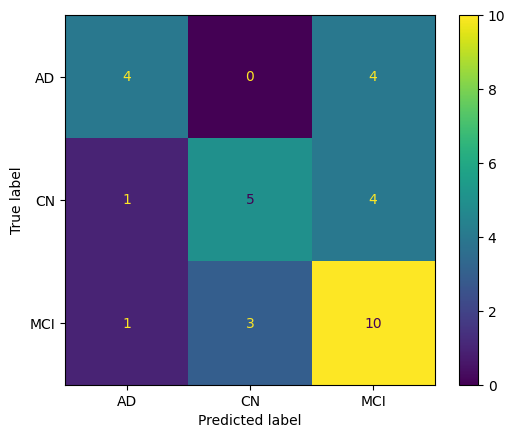
\includegraphics[width=\textwidth]{./imgs/resultados/coronal/CN_MCI_AD_cm_CORONAL}
        \caption{Comparativa CN-MCI-AD. }
        \label{fig:mc-coronal-cn-mci-ad}
    \end{subfigure}
    \caption{Matrices de confusión del plano Coronal.} \label{fig:mc-coronal}
\end{figure}

En una primera impresión, estos resultados son bastante buenos.
Al comparar entre CN y AD en el plano coronal se obtiene una precisión del 72\%, pero se observa que ha habido más
falsos negativos que falsos positivos.
En la clasificación entre CN, MCI y AD se obtiene una precisión del 59\% y un mayor número de falsos negativos, al
igual que en la clasificación de dos clases de este plano.

\subsection{Resultados del plano Sagital}\label{subsec:resultados-del-plano-sagital}

\begin{figure}[H]
    \centering
    \begin{subfigure}{0.4\textwidth}
        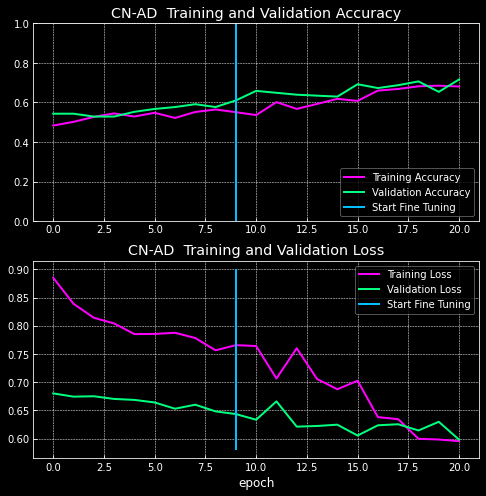
\includegraphics[width=\textwidth]{./imgs/resultados/sagittal/CN_AD_output_SAGITTAL}
        \caption{Comparativa CN-AD. }
        \label{fig:sagital-cn-ad}
    \end{subfigure}
    \hspace*{\fill}
    \begin{subfigure}{0.4\textwidth}
        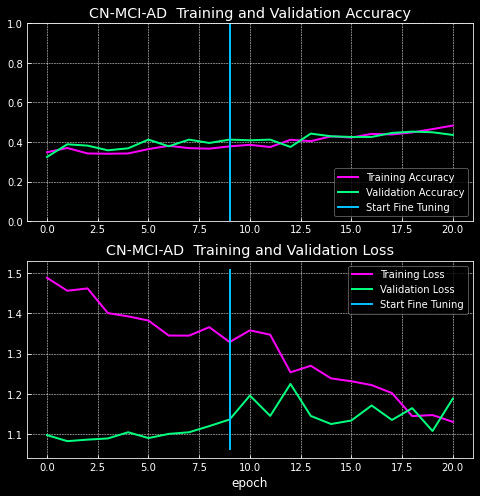
\includegraphics[width=\textwidth]{./imgs/resultados/sagittal/CN_MCI_AD_output_SAGITTAL}
        \caption{Comparativa CN-MCI-AD. }
        \label{fig:sagital-c-mci-ad}
    \end{subfigure}
    \caption{Evolución del modelo durante el entrenamiento: plano Sagital.} \label{fig:sagittal-model}
\end{figure}

\begin{table}[H]
    \centering
    \begin{tabular}{r r r r r}
        & precision & recall & f1-score & support \\
        AD & 0.64 & 0.67 & 0.65 & 21 \\
        CN & 0.30 & 0.27 & 0.29 & 11 \\
        & & & & \\
        accuracy &  &  & 0.53 & 32 \\
        macro avg & 0.47 & 0.47 & 0.47 & 32 \\
        weighted avg & 0.52 & 0.53 & 0.53 & 32 \\
    \end{tabular}
    \caption{Classification Report del plano Sagital. Comparativa CN-AD}
    \label{tab:cr-sagital-cn-ad}
\end{table}

\begin{table}[H]
    \centering
    \begin{tabular}{r r r r r}
        & precision & recall & f1-score & support \\
        AD & 0.48 & 0.62 & 0.54 & 16 \\
        CN & 1.00 & 0.10 & 0.18 & 10 \\
        MCI & 0.20 & 0.33 & 0.25 & 6 \\
        & & & & \\
        accuracy &  &  & 0.41 & 32 \\
        macro avg & 0.56 & 0.35 & 0.32 & 32 \\
        weighted avg & 0.59 & 0.41 & 0.37 & 32 \\
    \end{tabular}
    \caption{Classification Report del plano Sagital. Comparativa CN-MCI-AD}
    \label{tab:cr-sagital-cn-mci-ad}
\end{table}

\begin{figure}[H]
    \centering
    \begin{subfigure}{0.4\textwidth}
        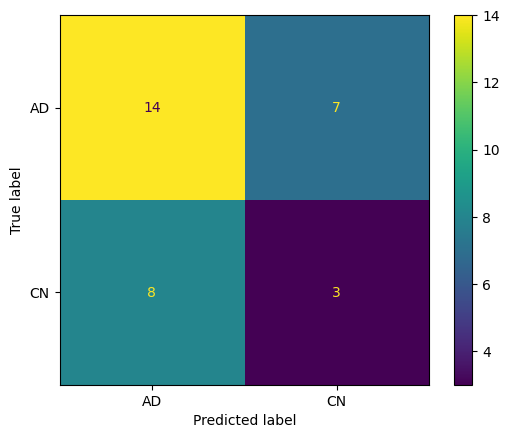
\includegraphics[width=\textwidth]{./imgs/resultados/sagittal/CN_AD_cm_SAGITTAL}
        \caption{Comparativa CN-AD. }
        \label{fig:mc-sagital-cn-ad}
    \end{subfigure}
    \hspace*{\fill}
    \begin{subfigure}{0.4\textwidth}
        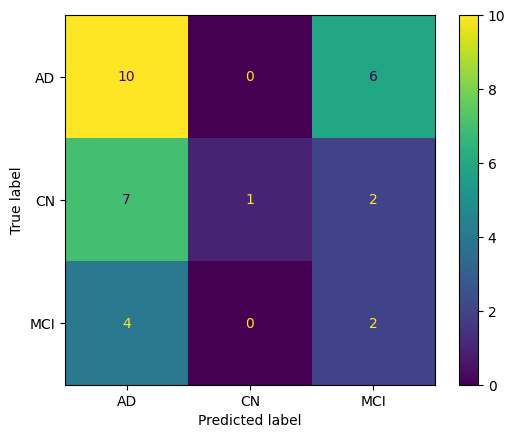
\includegraphics[width=\textwidth]{./imgs/resultados/sagittal/CN_MCI_AD_cm_SAGITTAL}
        \caption{Comparativa CN-MCI-AD. }
        \label{fig:mc-sagital-cn-mci-ad}
    \end{subfigure}
    \caption{Matrices de confusión del plano Sagital.} \label{fig:mc-sagittal}
\end{figure}

En el plano sagital se obtiene una precisión del 53\% en la clasificación entre CN y AD y un 40\% en la clasificación
entre CN, MCI y AD. Destacan en ambos una tendencia a etiquetar con más facilidad el tipo AD dando lugar a un mayor
número de falsos positivos que de falsos negativos.

\section{Conclusión}\label{sec:conclusion}

Para empezar hay que concluir que la evolución de los modelos durante el entrenamiento es muy similar.
En ninguno de los casos se obtiene una precisión mayor al 80\%.
Y además la tendencia de la función de pérdida es un indicador de que quizás haría falta un mayor número de muestras de
entrenamiento.
En este caso hemos utilizado el mayor número posible de las disponibles creando un dataset balanceado.
Sería interesante plantear una nueva vertiente en la que se mezclen biomarcadores de varias fuentes de datos como hacen
algunos estudios de la literatura, y como también se intentó en un principio en este proyecto, pero los requerimientos
de acceso a tales repositorios de datos es otro impedimento.

En cuanto a la pregunta que marca el objetivo de este proyecto. \textbf{¿Qué plano es mejor para el diagnóstico del
Alzheimer?} Claramente, teniendo en mente el valor de la precisión, en el \textbf{plano coronal} un mayor porcentaje
de datos han sido etiquetados de forma correcta que en el resto de planos tanto en la comparativa de 2 clases como
en la comparativa de 3 clases.

Además el plano coronal anatómicamente engloba las tres regiones más importantes del cerebro relacionadas con la EA:
el hipocampo, la corteza y los ventrículos.
Por lo tanto se puede concluir que sí es el mejor plano para el diagnóstico de la enfermedad.


